
A partir de este momento se comenzará a trabajar en modelos que verán la relación entre una variable continua, en este caso el precio de los artículos y una o mas variables independientes las cuales forman parte del data set original o se formaran a partir del enriquecimiento de los datos.
Antes de meterse de lleno en los métodos, cabe destacar que se realizó un proceso de Subset selection que iterativamente fue quitando pedictores poco relevantes y generando nuevos a modo de contar con el conjunto mas pequeño de ellos posible maximizando la ganancia en predicción. Este proceso se llevo acabo utilizando regresión lineal la cual se explicara en próximas secciones.
El conjunto de datos utilizado para los modelos esta compuesto por las siguientes variables:


\begin{itemize}
  \item \textbf{precio}: variable continua
  \item \textbf{medicion}: momento en el que se toma la medición 
  \item \textbf{baderaDescripcion}: nombre del punto de venta, cadena.
  \item \textbf{mCuadradoC}: variable categórica que indica el precio del metro cuadrado en  el barrio donde se esta vendiendo el producto, valores posibles: alto-medio-bajo
  \item \textbf{cantPtosVenta}: variable categórica que indica la cantidad de puntos de venta en el barrio donde se esta vendiendo el producto, valores posibles: alto-medio-bajo 
  \item \textbf{marca}: identificador de la empresa o tipo de producto
\end{itemize}



La siguiente sección se centrara en la generación de modelos para explicar y predecir la variable precio, también se realizara una evaluación e interpretación de los resultados obtenidos mediante los mismos.\\
La idea sera predecir el precio de los productos en base a ciertos predictores.
\cite{Stat_Learning}\\
La métrica elegida para evaluar los métodos es el Root Mean Square Error (RMSE), la cual calcula la diferencia entre los valores predichos y los observados. Se utilizará la proporción clásica para separar el dataset en $precios_train$ con el 70 \% de los datos seleccionados al azar para entrenamiento y $precios_test$ con el 30 \% restante para testear los modelos.



\section{Regresión lineal}

La regresión lineal es un método estadístico clasico que trata de modelar la relación entre una variable continua y una o mas variables independientes mediante el ajuste de una ecuación lineal. El método asume que las variables no están correlacionadas y funciona minimizando la suma de los cuadrados de los residuos (valor observado - valor predicho). 



\subsection{Simple}

%\begin{lstlisting}[language=R]
%modelo_lnS <- lm(formula = precio~banderaDescripcion, data=precios_train)
%\end{lstlisting}


Una primera aproximación de modelo lineal fue intentar explicar la variable precio por medio de la banderaDescripcion del punto de venta, si bien uno puede sospechar que solo conocer empresa que esta vendiendo un producto no alcanza para predecir o poder explicar el precio de un articulo dado, se tomo este modelo para tener de linea base para iterar en mas complejidad.\\

\begin{figure}[h]
\centering
\fbox{
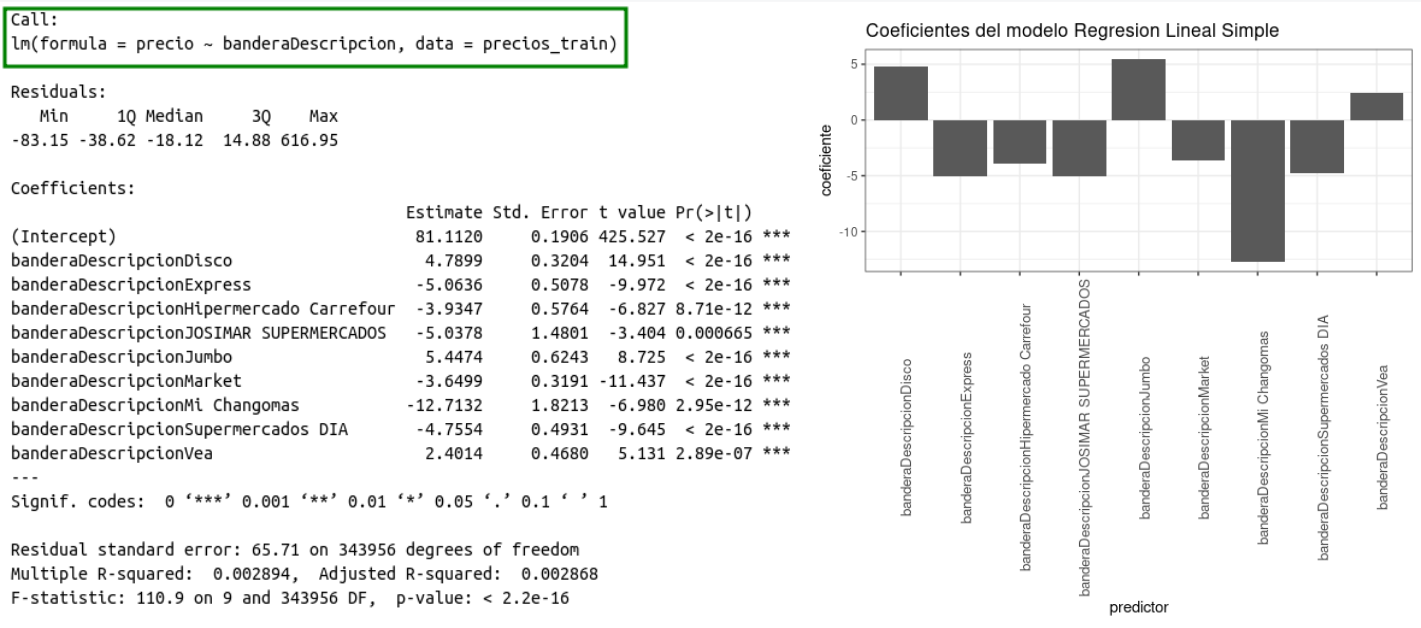
\includegraphics[width=0.95\textwidth]{img/ln_simple_full.png}
}%
\caption{Regresion lineal simple}
\label{ln_simple_full}
\end{figure}



Para evaluar este modelo revisaremos en detalle los siguientes puntos pero antes mencionando que el p-valor de todo el modelo obtenido es chico (menor a 0.05), lo cual refleja que es estadísticamente significativo.\\

\begin{itemize}
	\item Se observa que el valor del Intercept es de \$81.1120 , que se corresponde a la bandera COTO la cual si se compara con algunas de las variables dummy creadas a partir del resto de las banderas, se puede evidenciar que por ejemplo el valor de Disco sobre Coto es 4.7899
	
	\item Como antes se mencionó se obtuvo un p-value: < 2.2e-16 lo cual indica que significatividad estadística y todas las variables dummy creadas son también estadísticamente significativas. 
    
    \item El valor de R2 Ajustado es de 0.002868 lo cual indica que el modelo no esta siendo muy eficiente al predecir el precio de los productos basandose unicamente en el negocio que los comercializa en los datos de entrenamiento.\\
    Cabe destacar nuevamente que este modelo simples es muy basico, ya que se prendente entender como se explica la variabilidad del precio solo con una variable, así que sirven solo de punto de partida para tener una base a partir de la cual empezar a iterar en complejidad.
\end{itemize}
	
\subsubsection{Evaluación}
Como se comentó previamente se realiza una predicción del 30\% de los datos seleccionados para test con el modelo entrenado, obteniendo:\\
\textbf{Error (rmse) de test: 65.4811}

\subsection{Compuesto}


Para realizar una análisis mas rico para una variable precio es evidente que no basta con una sola variable, ya que el precio no es formado solamente por una de ellas sino por una conjunción de las mismas, por lo que se propone un modelo lineal compuesto donde entren en juego todas las variables que se habían definido al comienzo de la sección, a continuación de ira analizando el modelo compuesto y comprándose con el simple antes calculado.\\



\subsection{Estudio de p-value}

Lo primero que se quiere estudiar es la significancia del modelo, y de las covariables para entender cuantas de ellas son o no significativas, ya que al tener múltiples variables y que cada una de ellas ha generado variables dummy resuelta conveniente realizar el análisis en un gráfico de las variables con p-value mayor del total de las 306:\\



\begin{figure}[h]
\centering
\fbox{
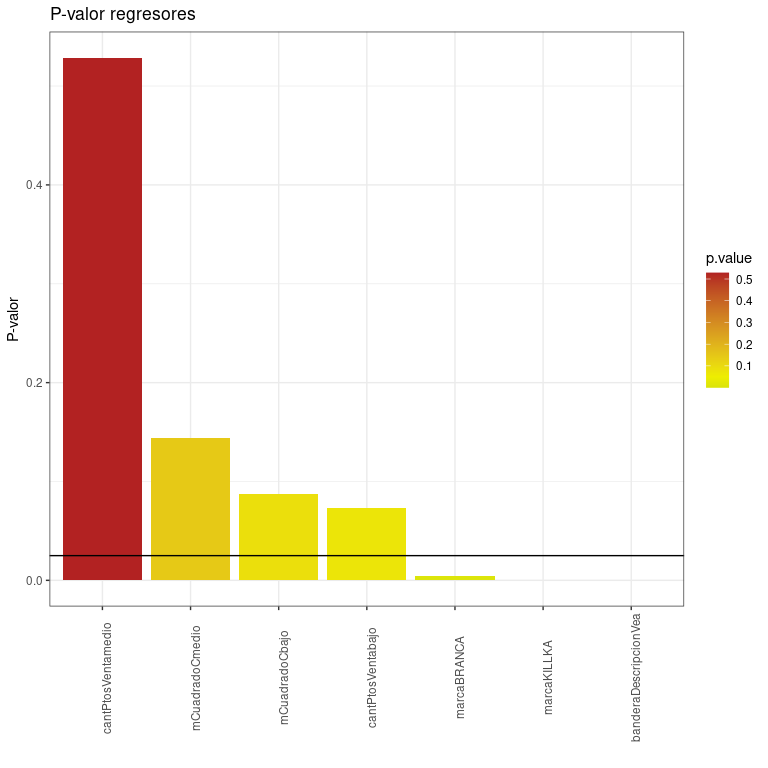
\includegraphics[width=0.7\textwidth]{img/pvalue_regresores.png}
}%
\caption{p-value regresores}
\label{p-value}
\end{figure}






En lineas generales podemos encontrar un p-value: < 2.2e-16 para el test, y la gran mayoría de las covariables tienen un valor de significancia adecuado.
Solo 4 de ellas, $cantPtosVentamedio$ $mCuadradoCmedio$, $mCuadradoCbajo$, $cantPtosVentabajo$ no tienen un p-value suficientemente bajo como para ser estadísticamente significativas en explicar la variabilidad de precio.\\
Cabe destacar que estas 4 variables, son parte de variables dummy que creo el modelo al generar la regresión ya que los valores de las variables orígenes eran categóricas multivaluadas.



\subsection{Estudio del residuo}

Los residuos (o errores) son la diferencia entre los valores observados y los valores que predice el modelo, con lo cual se espera que estos valores sean lo mas cercano a cero posibles, a menor residuo menor es la diferencia entre lo que esta prediciendo el modelo y el valor observado.\\
Con lo cual se buscara realizar un estudio del promedio de los residuos de ambos modelos para poder compararlos:\\



\begin{center}
 \begin{tabular}{||c c||} 
 \hline
    Residuo modelo linea simple & Residuo modelo linea múltiple \\ 
 \hline
 1.062773e-12 & -1.871219e-11 \\
 \hline
 \hline
\end{tabular}
\end{center}

Como se muestra en la tabla, la media de los residuos correspondientes al modelo lineal múltiple son de un orden de magnitud menor que los del modelo lineal simples.\\

En la siguiente comparación de gráficos podemos ver los polígonos dibujados por los residuos lo cual ayudara a entender la dispersión de los mismos, un mejor modelo esta asociado a una menor dispersión:


\begin{figure}[h]
\centering
\fbox{
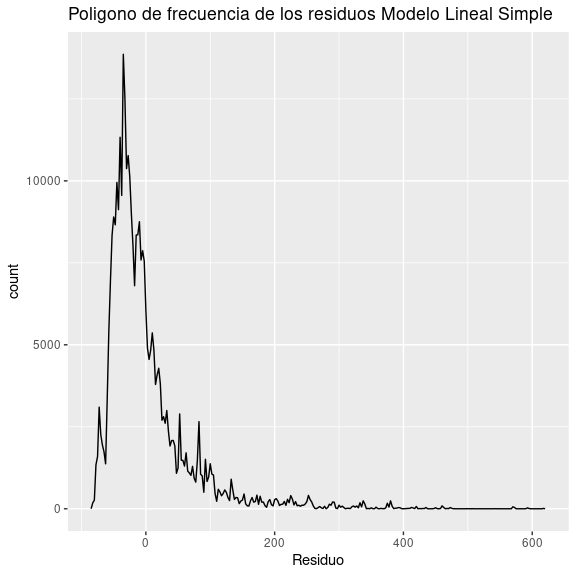
\includegraphics[width=0.45\textwidth]{img/ln_simple_poligono.png}
}%
\hspace{0.25cm}%
\fbox{
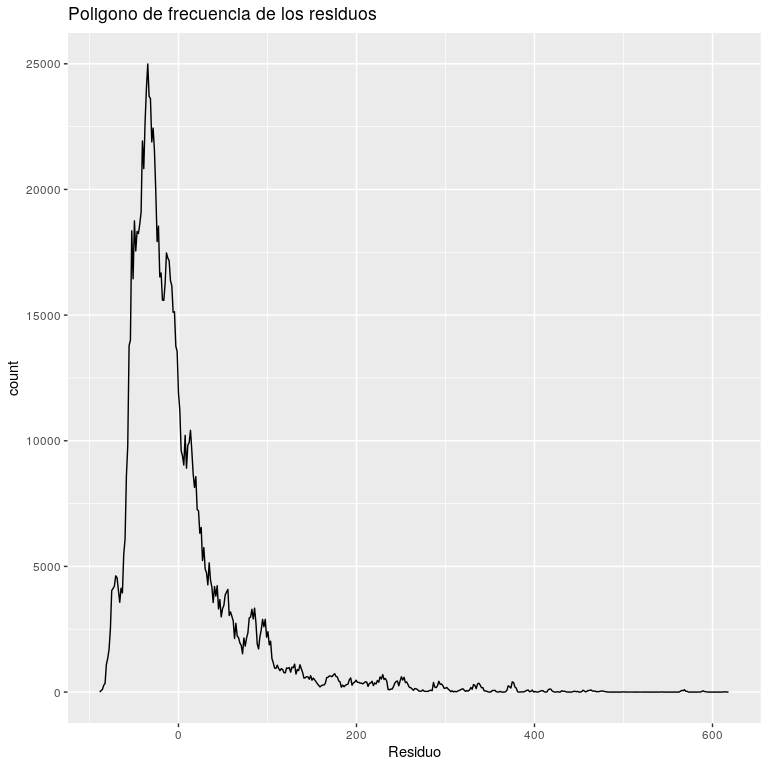
\includegraphics[width=0.45\textwidth]{img/ln_comp_poligono.png}
}
\caption{Comparación polígonos de los residuos}
\label{poligonos_comparativa}
\end{figure}


Se puede ver claramente por la escala, que la dispersión del modelo compuesto es mucho mas acotado que el del modelo simple, el cual presenta mayor dispersión.\\



A continuación en el análisis de los residuos se vera si los mismos siguen una distribución teórica N(0,1), a mejor adaptación de la curva de los residuos a esta distribución mejor sera el modelo.
Luego, se grafican ambos residuos:




\begin{figure}[h]
\centering
\fbox{
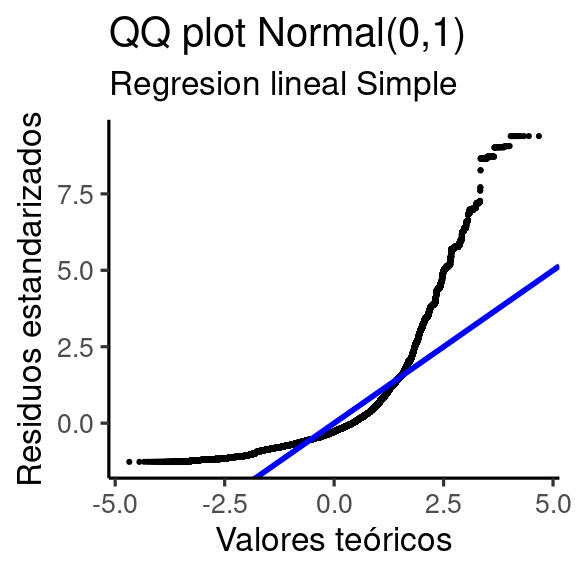
\includegraphics[width=0.45\textwidth]{img/ln_simple_qqplot.png}
}%
\hspace{0.25cm}%
\fbox{
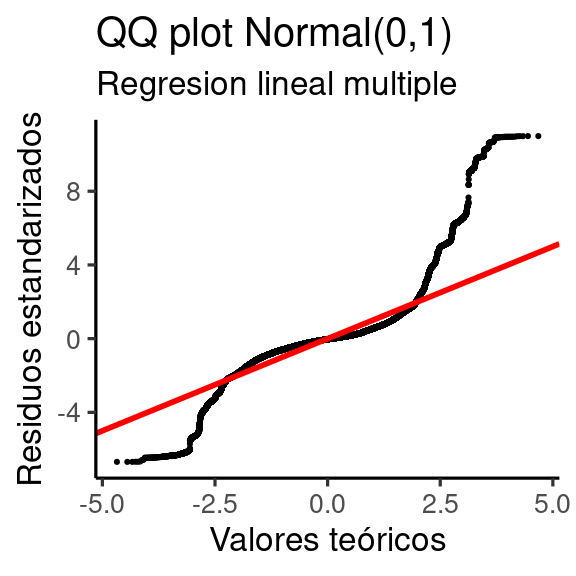
\includegraphics[width=0.45\textwidth]{img/ln_comp_qqplot.png}
}
\caption{Comparación QQ plots}
\label{qqplots_comparativa}
\end{figure}




Lo que se observa en este gráfico, es que si bien en los extremos la tendencia es alejarse de la recta y ninguno de los modelos se pega bien a la misma, los valores medios están mucho mas pegados a ella en el modelo compuesto que en el simple. \\

En una ultima corporación gráfica se estudiara la estructura de los residuos, la cual a mas definida y solida determinará un mejor modelo.



\begin{figure}[h]
\centering
\fbox{
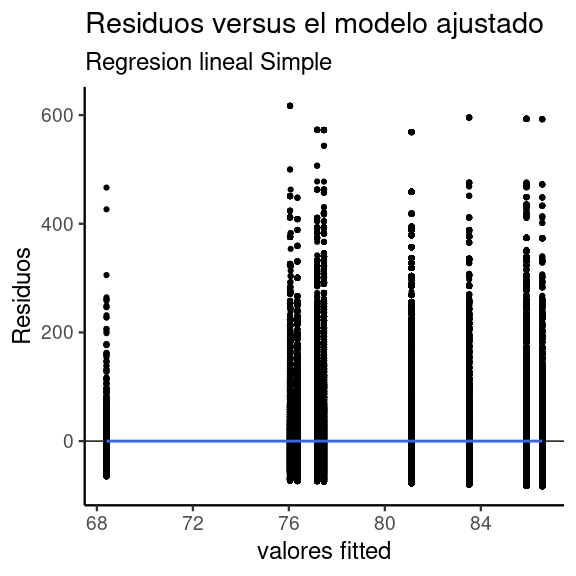
\includegraphics[width=0.45\textwidth]{img/ln_simple_resVsmodelo.png}
}%
\hspace{0.25cm}%
\fbox{
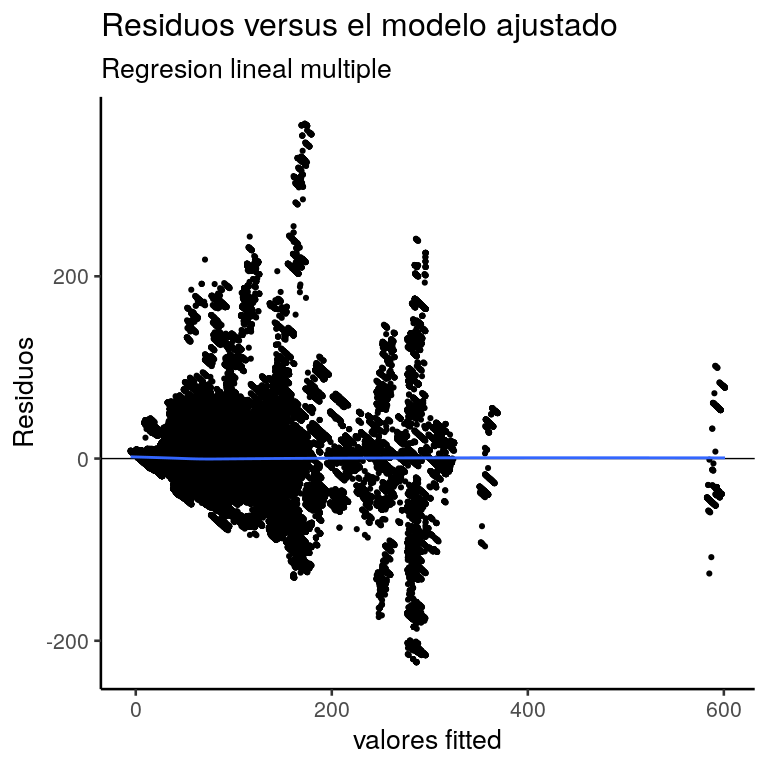
\includegraphics[width=0.45\textwidth]{img/ln_comp_resVsmodelo.png}
}
\caption{Comparación estructura de los residuos}
\label{estructura_comparativa}
\end{figure}


Si bien ninguno de los dos modelos presenta una estructura definida, se evidencia que para el primer modelo la formación de estructura es mucho menor que para el segundo, esto esta indicando que una parte sistemática del fenómeno se esta perdiendo, lo cual indica que el modelo no esta funcionando como se esperaría.\\


Por ultimo resta compara la suma de cuadrados residuales, R2 ajustados (ya que hay mas de una covariable), en la siguiente tabla se muestran los resultados obtenidos:\\


\begin{center}
 \begin{tabular}{||c c||} 
 \hline
    R2 ajustado lineal simple & R2 ajustado lineal múltiple \\ 
 \hline
 0.002867738 & 0.7404876 \\
 \hline
 \hline
\end{tabular}
\end{center}

Se observa que para el caso del segundo modelo múltiple, el R2 ajustado considerablemente mas alto y por consiguiente expresando un mejor modelo.

\subsubsection{Evaluación}
\textbf{Se obtiene: Error (rmse) de test: 33.4335}\\


Por todo lo anterior estudiado los resultados obtenidos, se puede concluir hasta este punto que el mejor modelo es el expresado por el modelo lineal múltiple.\\


Si bien la regresión lineal simple o múltiple es un método estadístico super utilizado posee algunas carencias al momento de su ejecución, la primera es que se ve altamente perjudicada cuando se encuentran covariables o predictores correlacionados, otro problema es que incluye todos los predictores, ya que no tiene capacidad de seleccionar algunos de ellos. Si el caso fuera en que todos aportan información relevante no habría mayores problemas, el inconveniente surge cuando hay un grupo, en especial considerable, de los mismos que no aporten información relevante lo cual disminuye su capacidad predictiva, por ultimo no logran un buen ajuste cuando la cantidad de predictores supera al numero de observaciones (este ultimo no es el caso de los datos que se están estudiando).\\
En la próxima sección se estudiará y trabajará con otro tipo de modelos los cuales traen una solución al hecho de poder elegir que predictores formaran parte del modelo y cuales no.







%%%%%%%%%%%%%%%%%%%%%%%%%%%%%%%%%%%%%%%%%%%%%%%%%%%%%%%%%%%%%%%%%%%%%%%%%%%%%%%%%%%%%%%%%%%%%%
%%%%%%%%%%%%%%%%%%%%%%%%%%%%%%%%%%%%%%%%%%%%%%%%%%%%%%%%%%%%%%%%%%%%%%%%%%%%%%%%%%%%%%%%%%%%%%
%%%%%%%%%%%%%%%%%%%%%%%%%%%%%%%%%%%%%%%%%%%%%%%%%%%%%%%%%%%%%%%%%%%%%%%%%%%%%%%%%%%%%%%%%%%%%%
%%%%%%%%%%%%%%%%%%%%%%%%%%%%%%%%%%%%%%%%%%%%%%%%%%%%%%%%%%%%%%%%%%%%%%%%%%%%%%%%%%%%%%%%%%%%%%




\section{Regularización}

Las técnicas de regularización o shrinkage son muy útiles cuando se trabaja con un set de datos que tiene una gran cantidad de variables las cuales podrían introducir gran variabilidad a las estimaciones de los parámetros. En el caso estudiado hasta el momento si bien no hay gran cantidad de variables, si se generan dummies y termina habiendo mas de 300 covariables, se realizara un modelado con dos regresores clásicos para probar si este tipo de modelo es mejor o no para predecir el precio de los productos.\\
En esta sección se analizaran dos tipos de regresores, \textbf{Lasso} y \textbf{Ridge} el primero correspondiente $\alpha$=1 y el segundo a $\alpha$=0, se hará una comparativa entre ambos igual que antes para unificar las explicaciones y los gráficos.\\
Cabe señalar que lo que diferencia entre estos métodos de regularización y los métodos lineales antes empleados, es que estas regularizaciones fuerzan a que los coeficientes de los predictores tiendan a cero, minimizando así el riesgo de overfitting, reduciendo varianza, atenuado el efecto de la correlación entre predictores y reduciendo la influencia en el modelo de los predictores menos relevantes.
Esta penalización esta controlada por el parámetro $\lambda$. Cuando $\lambda$=0 la penalización es nula y los resultados son equivalentes a los obtenidos por mínimos cuadrados, cuando $\lambda$=infinito todos los coeficientes son cero, lo que equivale al modelo sin ningún predictor (modelo nulo).\\
La elección del parámetro $\lambda$ adecuado es parte del estudio que se realizará mediante cross validation con un k=5 para buscar el óptimo y así computar el modelo con el parámetro optimizado.\\
Una variante a los modelos lineales antes aplicados, es que la librería glmnet() \cite{glmnet} requiere de una una matriz x con el valor de los predictores y un vector y con la variable respuesta, esto se puede obtener fácilmente con la funcion model.matrix()



\subsection{Lasso vs Ridge}

Si bien ambos modelos son muy similares Lasso, al igual que Ridge, fuerza a que las estimaciones de los coeficientes de los predictores tiendan a cero. La diferencia es que Lasso puede fijar algunos de ellos en cero, lo que potencia la reducción de la varianza.
Como contra parte Lasso es mas inestable ante presencia de correlaciones ente las covariables.


\subsection{Selección de $\lambda$}


Lo primero que se buscara es el gráfico de los coeficientes a medida que se va incrementando el valor de $\lambda$ para ambos modelos, la función glmnet()\cite{glmnet} guarda en una matriz los coeficientes de la regresión para cada valor de $\lambda$, lo cual permite graficar dicha evolución:



\begin{figure}[h]
\centering
\fbox{
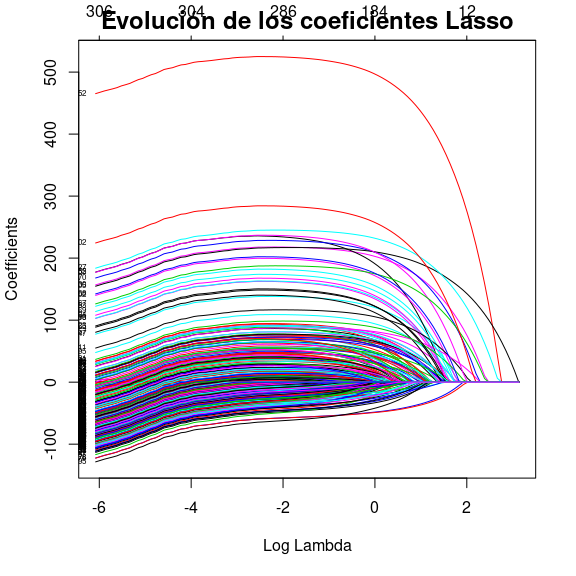
\includegraphics[width=0.45\textwidth]{img/lasso_coef.png}
}%
\hspace{0.25cm}%
\fbox{
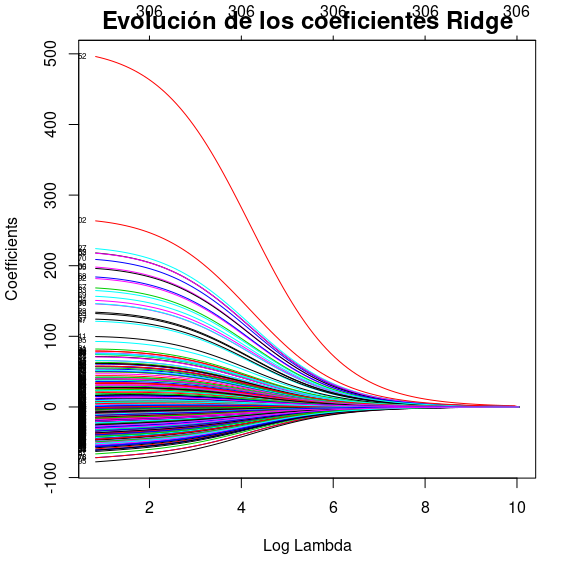
\includegraphics[width=0.45\textwidth]{img/ridge_coef.png}
}
\caption{Coeficientes según $\lambda$}
\label{coeficientes}
\end{figure}


Como expresan los gráficos, los coeficientes en ambos modelos se van haciendo mas pequeños a medida que se incrementa el valor de $\lambda$ y a su vez la regularización es mayor.\\
Con el fin de identificar el valor de $\lambda$ que da lugar al mejor modelo, se puede recurrir a Cross-Validation, como se hará a continuación.\\



\begin{figure}[h]
\centering
\fbox{
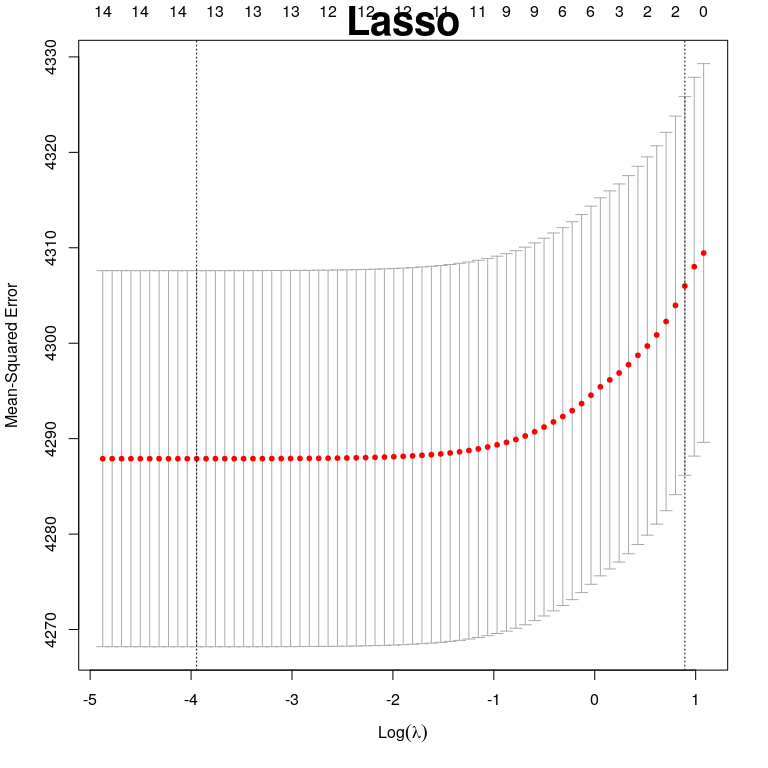
\includegraphics[width=0.45\textwidth]{img/lasso_cv.png}
}%
\hspace{0.25cm}%
\fbox{
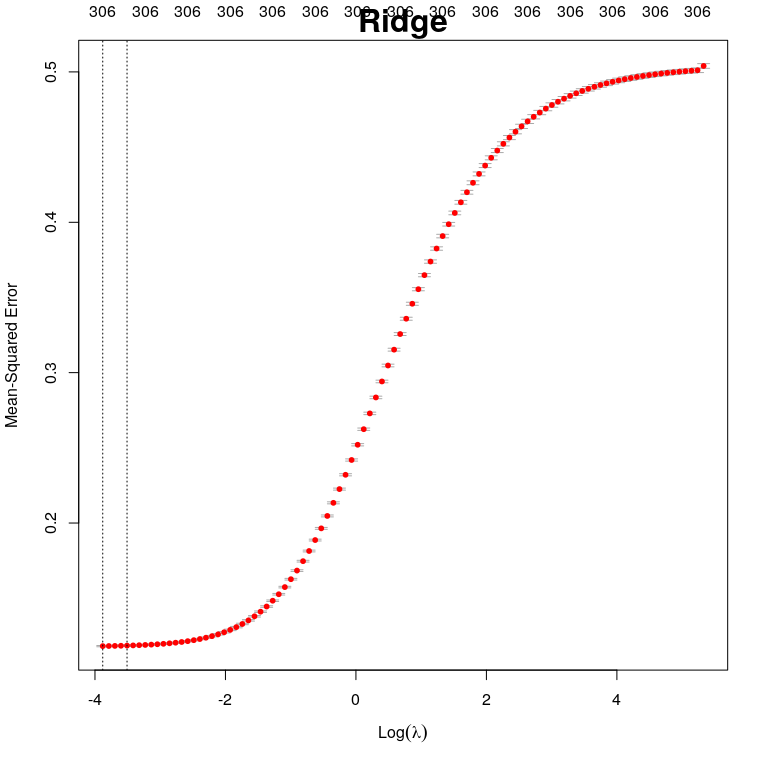
\includegraphics[width=0.45\textwidth]{img/ridge_cv.png}
}
\caption{Evolución $\lambda$}
\label{lambda}
\end{figure}



Los gráficos muestran el MSE (Mean Square Error) para cada valor de $\lambda$ junto con la barra de error correspondiente, la cual en ambos casos es muy pequeña. Se marcan dos valores de $\lambda$ específicos, el valor con el que se consigue el menor error y el valor con el que se consigue el modelo mas sencillo que se aleja a menos de 1 de desvío estandar del mínimo MSE posible. \\
También el gráfico evidencia la media del MSE con su limite superior e inferior y la cantidad de variables que sobreviven para cada valor de lambda.\\
Se volverá a correr los modelos pero esta ves con los valores min de $\lambda$ óptimos calculados.\\




\begin{center}
 \begin{tabular}{||c c c c||} 
 \hline
    Lasso $\lambda$ min & Lasso $\lambda$ 1se & Ridge $\lambda$ min & Ridge $\lambda$ 1se  \\ 
 \hline
    0.002289825	 & 0.01014535 & 2.289825 & 4.001535\\
 \hline
 \hline
\end{tabular}
\end{center}



Se volverán a correr ambos modelos ahora con el valor de $\lambda$ mínimo, y se estudiara cuantas variables sobreviven en cada caso, el deviance \cite{modelos} explicado por cada modelo y el resultado de la predicción.


\begin{center}
 \begin{tabular}{||c c c c||} 
 \hline
    Lasso \#variables & Lasso deviance & Ridge \#variables & Ridge deviance  \\ 
 \hline
    306 & 0.7391 & 306 & 0.7362\\
 \hline
 \hline
\end{tabular}
\end{center}



La cantidad de variables que sobreviven tanto para Lasso como para Ridge son 306, no se muestra una diferencia en este punto, el deviance que compara el modelo generado contra un hipotético modelo ideal es algo mejor en Lasso lo que podría pre suponer que obtendremos una mejor predicción.\\


\subsubsection{Evaluación}

\textbf{Lasso se obtiene: Error (rmse) de test: 33.5336}\\
\textbf{Ridge se obtiene: Error (rmse) de test: 33.7091} \\






\newpage
\section{Comparación de Modelos}

A continuación se comparan los resultados entre los 4 modelos estudiados en búsqueda de cual es el mas adecuado de todos.

\begin{figure}[h]
\centering
\fbox{
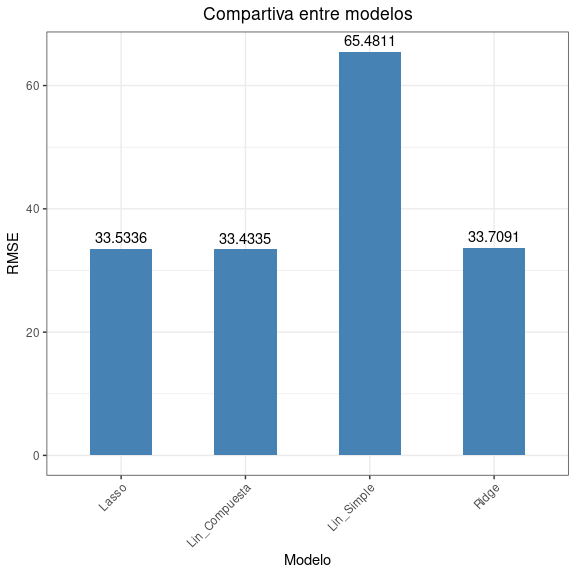
\includegraphics[width=0.6\textwidth]{img/Comprativa_modelos.png}
}%
\caption{Comparativa}
\label{comparativa}
\end{figure}


Como se puede ver el modelo lineal compuesto o múltiple es quien obtuvo el mejor resultado seguido muy de cerca por el modelo que utilizó el regresor Lasso y luego el regresor Ridge. Por ultimo se ubica la regresión lineal simple. 





